\subsubsection{Dijkstra - Caminho Mínimo com Pesos Não Negativos}
O algoritmo de Dijkstra encontra o caminho mais curto a partir de um nó origem
para todos os outros nós em um grafo com arestas de pesos não negativos. Ele
utiliza uma Fila de Prioridade (\textit{Min-Heap}) para explorar sempre o nó
mais próximo que ainda não foi totalmente processado, garantindo uma abordagem
gulosa e eficiente. Sua complexidade é: $\mathcal{O}(E \log(V))$

\paragraph{Pseudo-Código: }\mbox{}\\
\begin{algorithm}[H]
	\SetAlgoLined
	\SetKwFunction{Dijkstra}{Dijkstra}
	\SetKwProg{Fn}{Função}{:}{}

	\Fn{\Dijkstra{$inicio, adj$}}{
		$dist \gets$ array de distâncias inicializado com $\infty$\;
		$pq \gets$ nova FilaDePrioridade()\;
		$dist[inicio] \gets 0$\;
		$pq.push((0, inicio))$\;

		\While{\text{enquanto } $pq$ \text{ não vazia}}{
			$(d, u) \gets pq.top()$; $pq.pop()$\;

			\Se{$d > dist[u]$}{
				\text{continua para a próxima iteração}\;
			}

			\ParaCada{$(peso, v) \in adj[u]$}{
				\Se{$dist[u] + peso < dist[v]$}{
					$dist[v] \gets dist[u] + peso$\;
					$pq.push((dist[v], v))$\;
				}
			}
		}
	}
	\caption{Algoritmo de Dijkstra}
\end{algorithm}

Veja o Dijkstra funcionando, encontrando o caminho mínimo a partir do nó 1:\\
\vspace{0.5cm} \noindent % Garante que não haja recuo de parágrafo indesejado
\begin{minipage}[t]{0.31\textwidth}
	\centering
	\textbf{Passo 1: Início}\\
	\vspace{0.2cm}
	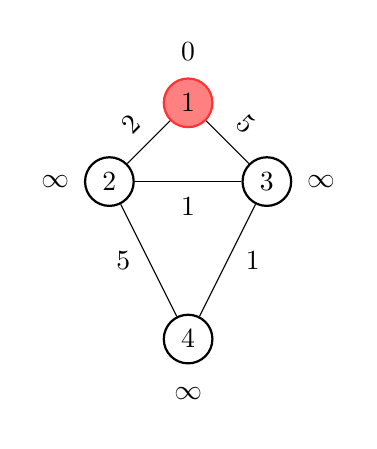
\begin{tikzpicture}[every node/.style={circle, draw, minimum size=0.5cm, thick}, visited/.style={fill=gray!30}, current/.style={fill=red!50, draw=red!80}]
		\node[current, label=above:{$0$}] (1) at (0, 1) {1};
		\node[label=left:{$\infty$}] (2) at (-1, 0) {2};
		\node[label=right:{$\infty$}] (3) at (1, 0) {3};
        \node[label=below:{$\infty$}] (4) at (0, -2) {4};
        
		\draw (1) -- node[above, sloped, draw=none, fill=none] {2} (2);
		\draw (1) -- node[above, sloped, draw=none, fill=none] {5} (3);
		\draw (2) -- node[below, draw=none, fill=none] {1} (3);
        \draw (3) -- node[right, draw=none, fill=none] {1} (4);
        \draw (2) -- node[left, draw=none, fill=none] {5} (4);
	\end{tikzpicture}

	\vspace{0.2cm}
	\footnotesize
	\raggedright
	Distância de 1 é 0. Outros são $\infty$. Fila: [(0, 1)].
\end{minipage}
\hfill
\begin{minipage}[t]{0.31\textwidth}
	\centering
	\textbf{Passo 2: Expandindo 1}\\
	\vspace{0.2cm}
	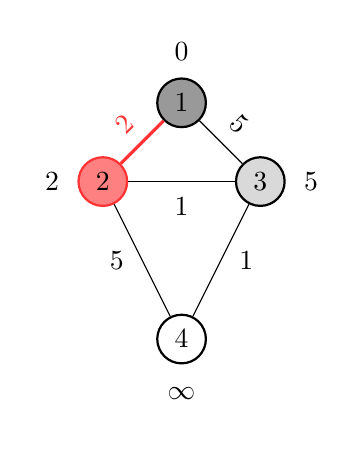
\begin{tikzpicture}[every node/.style={circle, draw, minimum size=0.5cm, thick}, visited/.style={fill=gray!30}, current/.style={fill=red!50, draw=red!80}, finished/.style={fill=gray!80}]
		\node[finished, label=above:{$0$}] (1) at (0, 1) {1};
		\node[current, label=left:{$2$}] (2) at (-1, 0) {2};
		\node[visited, label=right:{$5$}] (3) at (1, 0) {3};
        \node[label=below:{$\infty$}] (4) at (0, -2) {4};
		\draw[very thick, red!80] (1) -- node[above, draw=none, fill=none, sloped] {2} (2);
		\draw[visited] (1) -- node[above, sloped, draw=none, fill=none] {5} (3);
		\draw (2) -- node[below, draw=none, fill=none] {1} (3);
        \draw (3) -- node[right, draw=none, fill=none] {1} (4);
        \draw (2) -- node[left, draw=none, fill=none] {5} (4);
	\end{tikzpicture}

	\vspace{0.2cm}
	\footnotesize
	\raggedright
	Tira 1. Relaxa arestas. $dist[2]=2$, $dist[3]=5$. Fila: [(2, 2), (5, 3)].
\end{minipage}
\hfill
\begin{minipage}[t]{0.31\textwidth}
	\centering
	\textbf{Passo 3: Expandindo 2}\\
	\vspace{0.2cm}
	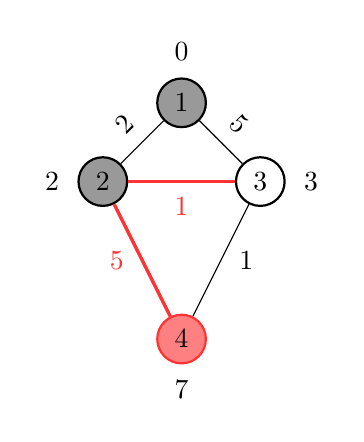
\begin{tikzpicture}[every node/.style={circle, draw, minimum size=0.5cm, thick}, visited/.style={fill=gray!30}, current/.style={fill=red!50, draw=red!80}, finished/.style={fill=gray!80}]
		\node[finished, label=above:{$0$}] (1) at (0, 1) {1};
		\node[finished, label=left:{$2$}] (2) at (-1, 0) {2};
		\node[label=right:{$3$}] (3) at (1, 0) {3};
        \node[current, label=below:{$7$}] (4) at (0, -2) {4};
        \draw[very thick, red!80] (2) -- node[left,fill=none, draw=none] {5} (4);
        \draw (3) -- node[right, draw=none, fill=none] {1} (4);
		\draw[finished] (1) -- node[above, sloped, draw=none, fill=none] {2} (2);
		\draw[visited] (1) -- node[above, sloped, draw=none, fill=none] {5} (3);
		\draw[very thick, red!80] (2) -- node[below, draw=none, fill=none] {1} (3);
	\end{tikzpicture}

	\vspace{0.2cm}
	\footnotesize
	\raggedright
	Tira 2. $2 + 1 < 5$. Atualiza $dist[3]=3$. $2+5 < \infty$, atualiza $dist[4] = 7$. Fila: [(3, 3), (5, 3), (7, 4)].
\end{minipage}
\newpage
\begin{center}
	\textbf{Passo 4: Expandindo 3}\\
	\vspace{0.2cm}
	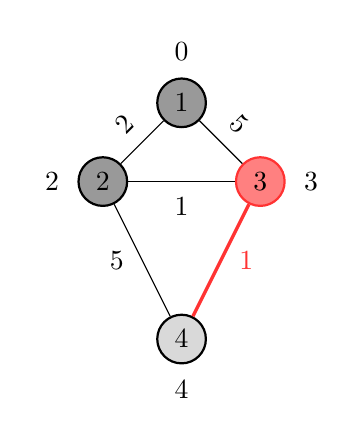
\begin{tikzpicture}[every node/.style={circle, draw, minimum size=0.5cm, thick}, visited/.style={fill=gray!30}, current/.style={fill=red!50, draw=red!80}, finished/.style={fill=gray!80}]
		\node[finished, label=above:{$0$}] (1) at (0, 1) {1};
		\node[finished, label=left:{$2$}] (2) at (-1, 0) {2};
		\node[current, label=right:{$3$}] (3) at (1, 0) {3};
        \node[visited, label=below:{$4$}] (4) at (0, -2) {4};
        
		\draw (1) -- node[above, sloped, draw=none, fill=none] {2} (2);
		\draw (1) -- node[above, sloped, draw=none, fill=none] {5} (3);
		\draw (2) -- node[below, draw=none, fill=none] {1} (3);
        \draw [very thick, red!80] (3) -- node[right, draw=none, fill=none] {1} (4);
        \draw (2) -- node[left, draw=none, fill=none] {5} (4);
	\end{tikzpicture}

	\vspace{0.2cm}
	\footnotesize
	\raggedright
	Está visitando o vizinho de 3 (4). $dist[3]+peso(3\xrightarrow{}4) < dist[4]$, isto é $3+1 < 7?$, sim então: $dist[4]=dist[3]+1$.
\end{center}
Nesse momento, não faz sentido avaliar mais os valores ainda presentes na fila de prioridade, que seriam: [(5,3), (7,4)], pois eles não iriam melhorar nenhum resultado. Pois o caminho (5,3) significa que tem peso 5 pra chegar até 3, porém isso seria descartado pela linha
\begin{lstlisting}[language=C++]
    if d>dist[u]{ 
        continue; 
    }
\end{lstlisting}
Essa linha de código serve justamente para evitar analisar relaxamentos de arestas desnecessários. 

Ao finalizar o Dijkstra nosso vetor de distâncias calculou o seguinte: 

$dist[u]$ é a distância mínima entre a origem $s$ até $u$, lembrando que para o exemplo acima a origem foi o vértice 1, então $dist[2]$ é a menor distância entre de 1 até 2. Esse algoritmo pode ser modificado, possibilitando que recriemos o caminho (basta criar um novo vetor chamado $parent$ em que $parent[u]$ guarda o vértice que levou até $u$ no menor caminho, por exemplo $parent[4]=3$, pois o caminho minímo de $1 \xrightarrow{}4$ foi $1\xrightarrow{}2\xrightarrow{}3\xrightarrow{}4$
\newpage
\paragraph{Implementação: }\mbox{}\\
Vejamos a implementação do Dijkstra em Python e C++. Note o uso de \textit{heaps} para otimização.

\textbf{Python: }
\begin{lstlisting}[language=Python]
import heapq

def dijkstra(inicio, adj, n):
    dist = [float('inf')] * n
    dist[inicio] = 0
    pq = [(0, inicio)]
    
    while pq:
        d, u = heapq.heappop(pq)
        if d > dist[u]:
            continue
            
        for peso, v in adj[u]:
            if dist[u] + peso < dist[v]:
                dist[v] = dist[u] + peso
                heapq.heappush(pq, (dist[v], v))
                
    return dist
\end{lstlisting}

\vspace{0.3cm}
\textbf{C++:}
\begin{lstlisting}[language=C++]
vector<int> dijkstra(int inicio, int n, const vector<vector<pair<int, int>>>& adj) {
    vector<int> dist(n, 1e9);
    priority_queue<pair<int, int>, vector<pair<int, int>>, greater<pair<int, int>>> pq;
    
    dist[inicio] = 0;
    pq.push({0, inicio});
    
    while (!pq.empty()) {
        int d = pq.top().first;
        int u = pq.top().second;
        pq.pop();
        
        if (d > dist[u]) continue;
        
        for (auto edge : adj[u]) {
            int peso = edge.first;
            int v = edge.second;
            
            if (dist[u] + peso < dist[v]) {
                dist[v] = dist[u] + peso;
                pq.push({dist[v], v});
            }
        }
    }
    return dist;
}
\end{lstlisting}